\documentclass{article}[]
\usepackage[textwidth=15cm]{geometry}
\usepackage[table,xcdraw]{xcolor}
\usepackage{graphicx}
\usepackage{listings}
\usepackage{hyperref}
\usepackage{pdfpages}
\usepackage{csvsimple}
\usepackage{float}
\usepackage{csquotes}
\makeatletter
\newcommand\urlfootnote@[1]{\footnote{\url@{#1}}}
\DeclareRobustCommand{\urlfootnote}{\hyper@normalise\urlfootnote@}
\makeatother

\begin{document}
\title{Neural Networks Assignment 2}
\author{Group 35}
\maketitle
\lstset{
  basicstyle=\ttfamily,
  keywordstyle=\bfseries,
  language=Java,
  frame=single,
  aboveskip=11pt,
  belowskip=11pt,
  breaklines=true,
  breakatwhitespace=false,
  showspaces=false,
  showstringspaces=false,
  numbers=left,
  stepnumber=1,    
  firstnumber=1,
  numberfirstline=true
}

\section{Introduction}
This report discusses our results for the second assignment for the Neural Network course, given in spring 2018 at LIACS.
The main purpose of this assignment is to get familiar with the neural networks library \textit{Keras}\cite{chollet2015keras} written for \textit{python}\cite{van2011python}.

Section \ref{sec:mnist} focuses on using two different methods, namely \emph{Multilayer perceptron} (MLP) and \emph{Convolutional Neural Network} (CNN), to classify handwritten digits taken from the well known MNIST-Dataset\cite{mnist}.

%TODO
Section \ref{sec:seq} and \ref{sec:trans} are about natural language processing or the processing of arbitrary sequences / sentences. This is done using LSTM's and GRU's instead of plain Recurrent Neural Networks (RNN's)
Section \ref{sec:rnn} then uses plain RNN's to see if based on pure sequence / string input it is possible to teach a neural network to do basic calculations like addition and multiplication.

\section{MNIST-Classification with Keras}
\label{task-1}
% xxxxxxxxx – print top 3 “most misclassified” digits
% xxxxxxxx – how do you define “most misclassified”? 
% xxxxxxxx change the error function to MSE and rerun your experiments
%– to which extent are your results reproducible? In other words:
%what is the impact of “non-controllable” randomness?
%xxxxxxxxx apply mnist_mlp.py and mnist_cnn.py to a “randomly permutedversion” of the mnist dataset (pixels of all images permuted with help of a fixed random permutation of their indices)
\label{sec:mnist}
This section is about the classification of handwritten digits using the MNIST-Dataset.
For this we used the existing \textit{Keras}\cite{chollet2015keras}-examples called \textit{mnist\_mlp.py}\cite{kerasexamples} and \textit{mnist\_cnn.py}\cite{kerasexamples}.
In section \ref{example-scripts} we describe the model of these two scripts.


First we want to take a look at the three \emph{most misclassified digits}, see Section \ref{most-misclassified-digits}.
We define \textit{most misclassified} as follows: The samples where the probability of the $y_{true}$ label was the lowest.

After that we want to determine the impact of the used error function of these two nets.
Both the examples are using the \emph{categorical cross entropy} (CEE) error function.
In order to see how the performance of the nets change we repeated the experiments while using the \emph{mean squared error} function.
The findings are described in Section \ref{evaluation}.

To discover possible weaknesses of the MLP, we permuted both the training and the test samples using a fixed permutation matrix.
After that we run the same experiment again with the CNN and described the results in Section \ref{evaluation}.


\subsection{Example Scripts}
\label{example-scripts}

The model of the \emph{mnist\_mlp.py}, see Listing \ref{mnist-mlp}, script looks like the following:
As you can see, the script builds a sequential model with three \emph{Dense} layers and two \emph{Dropout} layers.
As activation function the \emph{rectified linear unit} is used for the first two Dense layers.
The output layer uses the \emph{softmax} activation function.
The Dropout layers helps preventing overfitting, by dropping samples during the training process.

The MLP net trains for a total of 20 epochs and has 669,706 trainable parameters .

\begin{lstlisting}[language=Python, label=mnist-mlp, caption={mnist\_cnn.py model}, captionpos=b]
model = Sequential()
model.add(Dense(512, activation='relu', input_shape=(784,)))
model.add(Dropout(0.2))
model.add(Dense(512, activation='relu'))
model.add(Dropout(0.2))
model.add(Dense(num_classes, activation='softmax'))
\end{lstlisting}

The sequential model of the \emph{mnist\_cnn.py}, see Listing \ref{mnist-cnn}, is more complicated and contains the following layers:
A convolutional 2D layer with a kernel size of (3, 3), which creates 32 feature maps in the size of (26, 26).
A second convolutional 2D layer with a kernel size of (3, 3), which creates 64 feature maps in the size of (24, 24).
The max pooling 2D layer reduces the size of the feature maps, by finding the highest value in a (2, 2) window and output it to the next layer.
The Flatten layer reduces the dimensionality to 1, in order to use two Dense layers afterwards.
Again the \emph{rectified linear unit} activation function is used everywhere, but in the output layer, where the \emph{softmax} function is used.
Also there are two Dropout layers, to prevent overfitting.

% dropout layers erwähnen
The CNN trains for a total of 12 epochs and has 1,199,882 trainable parameters, which is quite a lot and explains the long runtime.

\begin{lstlisting}[language=Python, label=mnist-cnn, caption={mnist\_mlp.py model}, captionpos=b]
model = Sequential()
model.add(Conv2D(32, kernel_size=(3, 3),
                 activation='relu',
                 input_shape=input_shape))
model.add(Conv2D(64, (3, 3), activation='relu'))
model.add(MaxPooling2D(pool_size=(2, 2)))
model.add(Dropout(0.25))
model.add(Flatten())
model.add(Dense(128, activation='relu'))
model.add(Dropout(0.5))
model.add(Dense(num_classes, activation='softmax'))
\end{lstlisting}



\subsection{Most misclassified digits}
\label{most-misclassified-digits}
We run the examples scripts and tracked the three most misclassified digits of both the CNN and the MLP net.
Looking at figure \ref{fig:cnn} we can that the misclassifications of the CNN mostly seem to revolve around thin digits.
The first 9 is too thin, the 1 is barely visible and the 8 is too thin, too little and contains a noisy line.

\begin{figure}[H]
	\centering
	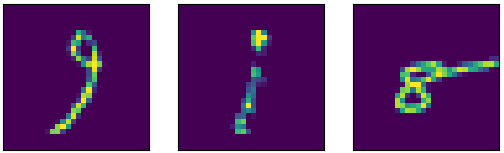
\includegraphics[width=0.5\linewidth]{img/cnn_categorial_cross_non_perm.png}
	\caption{Top three most misclassified digits with the CNN-CEE net}
	\label{fig:cnn}
\end{figure}

The three most misclassified digits of the MLP, shown in figure \ref{fig:mlp}, stand in stark contrast to that.
The left and the right sample seem to be very clearly identifiable.
One problem might be the thickness given that both samples are quite thick.
The middle one is easily identifiable by a human, but is very thin compared to the others, which might be the reason why it was misclassified.
Of course other reasons could have led to this result as well.

\begin{figure}[H]
	\centering
	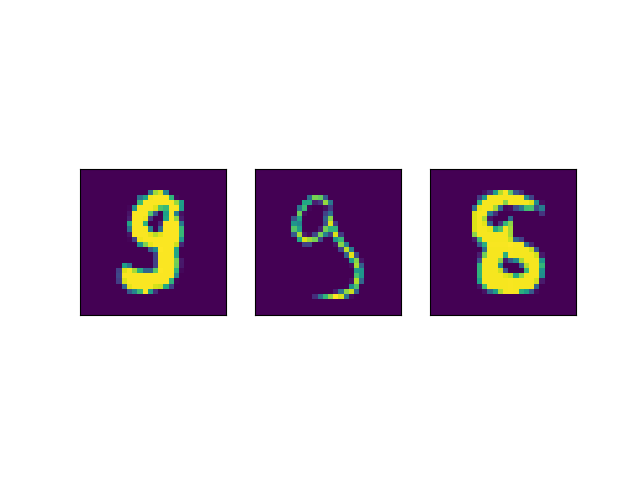
\includegraphics[width=0.5\linewidth]{img/mpl_categorial_cross_non_perm.png}
	\caption{Top three most misclassified digits with the MLP-CEE net}
	\label{fig:mlp}
\end{figure}

\subsection{Evaluation}
\label{evaluation}

In table \ref{table-1} you can see the amount of misclassified samples out of a total of 10000 test samples per experiment.
The rows describes the net type and the columns describe the error function and whether the permuted or the original data set was used.
It is evident, that CNN outperforms the MLP.

Both networks perform best with the cross-entropy error function.
The mean-squared error only slightly worsens the results of the MLP.
The CNN however, performs much worse using the mean squared error.

When looking at the results for the permuted data, we can see that it has a much greater impact on the CNN than on the MLP results.
It almost doubles the misclassified samples with the CNN, but doesn't affect the MLP results significantly.
This effect can be explained by the nature of the convolutional filters.
A convolutional filter \enquote{detects} features by looking at multiple information, in this case multiple pixels, at the same time.
By permutation the data, the feature recognition cannot work properly anymore, because it's important which pixels are next to each other.
The permutation will affect the results of the filters in an unpredictable way.

This problem doesn't occur with a plain MLP net, because every pixel is considered individuality.
As long as a pixel is moved to another place consistently over all images, it doesn't affect the behavior at all.


\begin{table}[H]
	\centering
	\begin{tabular}{|l|l|l|l|l|}
		\hline
		& \cellcolor[HTML]{C0C0C0}CEE & \cellcolor[HTML]{C0C0C0}CEE-P & \cellcolor[HTML]{C0C0C0}MSE & \cellcolor[HTML]{C0C0C0}MSE-P \\ \hline
		\cellcolor[HTML]{C0C0C0}MLP & \cellcolor[HTML]{FFFFFF}166 & 178                           & 169                         & 189                           \\ \hline
		\cellcolor[HTML]{C0C0C0}CNN & 77                          & 123                           & 149                         & 221                           \\ \hline
	\end{tabular}
	\caption{Amount of misclassified samples. CEE = cross-entropy error; MSE = mean-squared error, P = permutated sample}
	\label{table-1}
\end{table}

\subsection{Randomness impact}
To determine the possible impact of randomness upon accuracy of the recognition we run same tests again.
The results are shown in table \ref{table-2}.
As you can see, the results don't differ too much from the first runs.
The margin between the misclassified samples seems negligible.


\begin{table}[H]
	\centering
	\begin{tabular}{|l|l|l|l|l|}
		\hline
		& \cellcolor[HTML]{C0C0C0}CEE & \cellcolor[HTML]{C0C0C0}CEE-P & \cellcolor[HTML]{C0C0C0}MSE & \cellcolor[HTML]{C0C0C0}MSE-P \\ \hline
		\cellcolor[HTML]{C0C0C0}MLP & \cellcolor[HTML]{FFFFFF}154 & 160                           & 169                         & 174                           \\ \hline
		\cellcolor[HTML]{C0C0C0}CNN & 88                          & 128                           & 147                         & 216                           \\ \hline
	\end{tabular}
	\caption{Amount of misclassified samples. CEE = cross-entropy error; MSE = mean-squared error, P = permutated sample}
	\label{table-2}
\end{table}

\section{Text Generation}
\label{sec:seq}
This section deals with using  \emph{Long short-term memory} (LSTM) networks for natural language processing.
It presents the generation of text based on the learned data.
The text generation is based on the \textit{Keras}-example called \textit{lstm\_text\_generation.py}\cite{kerasexamples}.


\subsection{Script}
\label{textgen-script}
In this script a Nietzsche writing is used, the text is read and all $distinct\_characters$ are collected and enumerated.
After that the text is split up into \enquote{sentences}.
Sentences is in quotes, because the script uses the \emph{sliding window} technique. %TODO: Referenz für Sliding Window
This means we have a window of $window\_size$ characters, this window will be moved in every iteration by $step\_size$ characters.
This results in cut off words, but improves the contextualization between the sentences.
To feed the sentences to the network they are vectorized into a boolean representation.
The encoded data has the following shape:  \texttt{x=(sentence\_count, distinct\_character\_count)} and for 
\texttt{y=(sentence\_count, sentence\_length, distinct\_character\_count)}.

This data is then fed to the network.
At the end of every epoch, it generates text based on a random slice of text of the original input text.
With this \emph{seed} it will predict character by character.
This happens with a varying degree of diversity, meaning not using the most probable next character, but varying and hence enabling less probable characters to be used, with increasing diversity.
According to the author of the script, after 20 epochs text should start to sound coherent.
It also states, that increasing the size of the trained text should improve results.

\subsection{Experiments}
In order to evaluate the generation we run the following experiments
\begin{enumerate}
\item{Run the example-script as is}
\item{Run the example-script as is with increased sliding window size}
\item{Run the example-script as is with increased sliding window size with different input text}
\item{Run the example with different text input and use a GRU instead of LSTM}
\end{enumerate}

Our different text input are all books from Harry Potter combined.
The used book text was quite noisy, so we decided to clean it via a script.
We removed several orthography related characters and new lines.
This resulted in a $distinct\_characters$ drop to 37.
To compare, Nietzsche's text contains 52.
The adjusted input contains a much larger text corpus than the original input.
The cleaned version of all Harry Potter books contains around 6,14 million characters.
In comparison to Nietzsche's writings which consists of 600,901 characters.
This means a factor 10 increase of the training data.
We believe this will improve the results, given that less non fitting characters can be predicted and more training data is provided.

In addition we increased the sentence length to 100 instead of 40.
We set the $step\_size$ from 3 to 6.
We decided to adjust these parameters, because 40 characters seem to be too short.
In order to find a good length we looked up the average sentence length in the English language which is supposed to be 15-20 words\cite{cutts2013oxford}.
Also the average word length is approximately 5 characters\cite{shannon1951prediction}.
Combining that results in 100 characters per sentence ($20 * 5$).
We also expect a longer sequence length to improve the generated result, given that LSTM's use historical data well, and short sequences might already have dropped relevant previous context\cite{sundermeyer2013comparison}.

The last experiment uses a GRU instead of a LSTM, which is a bit simpler than the LSTM, but should yield similar results \footnote{\url{http://colah.github.io/posts/2015-08-Understanding-LSTMs/}}.



\subsection{Results}
% Nietzsche original
The script as is generates somewhat valid English words after 60 epochs of learning with a diversity of 0.5, see Listing \ref{nietzsche-low-diverse}.

%Nietzsche modifierd
When comparing the results of the vanilla script,  with the ones of the adjusted script, see Listing \ref{nietzsche-adjusted-low-diverse}, we can see that increasing the sliding window size does not seem to negatively affect the validity of the generated text.
However, the produced words only make sense individually.
They do not create meaningful sentences.
When increasing the diversity the results are getting worse and worse to the point where it becomes just random characters, hence we did not included it in the appendix.

% Harry Potter Vanilla (sliding window angepasst)
When changing the input text to the Harry Potter books, the LSTM (Listing \ref{harry-adjusted-low-diverse}) generated a coherent sounding sentence, after just 7 epochs, which is then followed by 140 characters of i's and other single characters.
Interestingly enough it then recovers producing normal words again.
Although it sounds grammatically well formed, the sentence does not make sense in what it says.

%GRU
The GRU  produces good results after just 1 epoch in the sense that the output only contains 7 invalid words and no character gibberish.
Also the words that are wrong always contains a substring of a valid word, but it gets invalidated by a wrong leading or trailing character.
The sentence has not as good of a grammatical structure as the LSTM.

During training we noticed a very strange behavior, where the generated text became worse with increasing epochs.
That's why we presented the output after just a few epochs.
This was unexpected, because the script claims after 20 epochs the text sounds coherent.
However in our results, the best text was produced after just 7 epochs and even just 1 epoch for the GRU, see Listings \ref{harry-adjusted-low-diverse} and \ref{harry-gru-low-diverse}.
The quality of the text was also deducible from the loss value during the training process.
For the shown results it was between 1 and 2.
After the next epoch of the good results, the loss values rose to 7 or 5, further training did lower the loss, but it never reached a value below 4.
Sentences with a loss value above 2 already look like pure gibberish (example in Listing \ref{harry-gru-gibberish})

\section{Text Translation}
\label{sec:trans}
In this section we want to focus on the translation of strings from a source to a target language.
For this we use the \emph{Keras} example script called \emph{lstm\_seq2seq.py} \cite{kerasexamples}.

\subsection{Script}
The script reads a text file in which every line represents a translation.
The first part is the source language, delimited by a tab character indicating the start of the target language.
The input gets processed in a similar way as the text generation script, see Section \ref{textgen-script}.
One of the changes is, that the representation of the sentences is encoded with floats instead of booleans.

The model consists of an encoder and a decoder model.
Both are LSTMs and are combined into one model in order to train the net.

In total the model trains for 100 epochs.

\subsection{Experiments}
In order to evaluate the translation we run the following experiments:

\begin{enumerate}
	\item{Run the example-script as is}
	\item{Run the example with English to Dutch translation}
\end{enumerate}

\subsection{Results}
We validate the translation for correctness by comparing the expectation with the prediction.
Source sentences can occur multiple times, hence for these we check if one of the possible translation matches.

% TODO: Fra -> Eng

% English -> Dutch
The English to Dutch translation is not very effective.
Only 1705 of 10,000 sentences are translated correctly.



\section{Addition and Multiplication}
\label{sec:rnn}
Our goal for this section is to train \emph{Recurrent Neural Networks} (RNNs) to do additions and multiplications by solely providing string sequences as data.

\subsection{Script}
The experiments are based on the Keras example script \textit{addition\_rnn.py}\cite{kerasexamples}.
The script generates 50,000 additions with solutions.
There is an question and an expectation array.
The questions are saved as string that look like the following:
\texttt{023+123}.
As you can short numbers are padded with zeros in front.
The same holds true for the expectation.

After generation, the samples get vectorized just like the data in section \ref{textgen-script}.


% TODO
The sequential model consists of two LSTM layers.
The first LSTM layer works as encoder which soutputs HIDDEN\_SIZE values.
The second LSTM layer works as decoder and returns all outputs so far.
Then a TimeDistributed layer is applied to densify every slice of the input from the encoder.

\subsection{Experiments}
For the evaluation we run two experiments:
\begin{enumerate}
	\item{Run the example-script as is}
	\item{Run the example-script using varying RNNs types and layer amounts for multiplication}
\end{enumerate}

For the multiplication we generated 270,000 training samples that look like the addition samples.
We also generate a test set of 1,000 samples, that are not included in the training set.
Because the multiplication is more complex than the addition, we decided to try out different types of RNNs, namely LSTMs and GRUs.
We also experiment with using five decoding layers instead of just one.
During the training we saved the model after every iteration to be able to evaluate the performance of the model over time.

\subsection{Results}
The addition script claims to have an accuracy of 99\% on a training set of 50,000 samples.
We ran the script and achieved full accuracy after just 42 iterations.
Because the results are already almost perfect we decided not to run further experiments on the addition.


%multiply
%TODO übergang besser machen
For the multiplication the results can be seen in Figure \ref{fig:multiply}.
The accuracy of the different nets are plotted at every iteration.
It is evident, that the additional decode layers have worsened the accuracy.
In addition, the runtime was much higher.
Thats why we decided to stop the learning process of the net, with the 5 LSTM decode layers at 77 iterations.
But nevertheless, the best accuracy for this net is already reached after 20 to 30 iterations.
The one layer GRU and LSTM nets are competing quite close, but the very best accuracy is reached by the LSTM at around 80 iterations.
The GRU also shows an interesting disadvantage in the graph: at some iterations accuracy drastically drops, but yet it always recovers.

\begin{figure}[H]
\centering
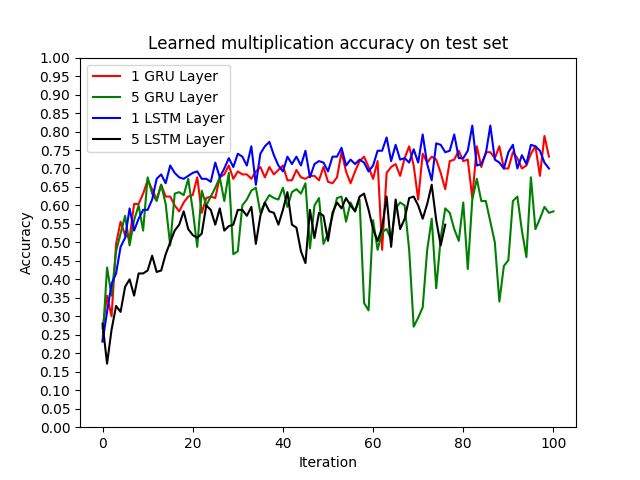
\includegraphics[width=1\linewidth]{img/multiply}
\caption{Evaluating multiplication accuracy on the test set using varying nets}
\label{fig:multiply}
\end{figure}

\section{Autoencoder}
\label{sec:autoencoder}
In this section we want to take a look on \emph{Autoencoders}.
For this purpose we encode MNIST digits to compress then.
Afterwards we decode them again in order to see how good the autoencoder works.
We also want to experiment with denoising images.
For that we apply random noisy pixel onto the original samples and try to denoise the sample afterwards.

The scripts are based on the \emph{The Keras Blog} entry \emph{Building Autoencoders in Keras}\footnote{https://blog.keras.io/building-autoencoders-in-keras.html}.

\subsection{Experiments}

\begin{enumerate}
	\item{deep vs. modified deep autoencoder}
	\item{convolutional vs. modified convolutional autoencoder}
	\item{convolutional denoising vs modified convolutional denoising autoencoder}
\end{enumerate}

\subsection{Results}




\appendix
\section{Text Generation}
\begin{lstlisting}[label=nietzsche-low-diverse, caption={riginal script with Nietzsche after 60 epochs and a diversity of 0.5}]
----- diversity: 0.5
----- Generating with seed: "emplation of the saint suggested to them"
emplation of the saint suggested to themselves to the intelligious sound of the pleasure, and their salver, there is a purpose is always at the person of power and necessary of mean will, as it is not the impudiated and conscience to which the world at all like the process of the sign of the self-destinct of the world the spirit, and in the consequent, as it will been discoverer of the scame of self european and secrecy and act of life 
\end{lstlisting}

\begin{lstlisting}[label=nietzsche-adjusted-low-diverse, caption={adjusted original script with Nietzsche after 60 epochs and a diversity of 0.5}]
----- diversity: 0.5
----- Generating with seed: "o their taste,
including the enmity and voltairean bitterness against religion (and all
that formerl"
o their taste,
including the enmity and voltairean bitterness against religion (and all
that formerly, the saits that
it was an inventives are more and the servits of the incaln man who is always the secre to himself? this is the most pain the probably made also a great wordsy
(or efor that it is always a strong to the ancient ruinssed his despaysved his actions and conscious the wean the boldaing, and may be exalled, which not we free spiritsked, and which is not
opinions and his own indepenced
\end{lstlisting}


\begin{lstlisting}[label=harry-adjusted-low-diverse, caption={adjusted original script with Harry Potter after 7 epochs and a diversity of 0.5}]
----- diversity: 0.5
----- Generating with seed: "t harry, never forget that what the prophecy says is only significant because voldemort made it so. "
t harry, never forget that what the prophecy says is only significant because voldemort made it so. hermione to hard burned the stairs and the words would hear the best of the window and looking out of the exterm in the field. i a n i do i i i i i i i i i d i i i i i p i i i i i i i i i i i i i i i i i i i i i i i i i i i i i i i i i i i i l n i do i i i i i i i f on the sirius was said harry, with the houses and some of his portrait and the neare, and a with him the third with a screaming and b
\end{lstlisting}


\begin{lstlisting}[label=harry-gru-low-diverse, caption={script with GRU and with Harry Potter as input after 1 epoch and a diversity of 0.5}]
----- diversity: 0.5
----- Generating with seed: " it was, he had just done serious magic, which meant that he was almost certainly expelled from hogw"
it was, he had just done serious magic, which meant that he was almost certainly expelled from hogwarting into the carry a scurred around that sitter her starter was as on the wand her face at that someth ye moaned that you cant they suppose to her harry happied her set of the carried of the of the carried the floor. expered and last that was connetter sumpration she case for hermione could he said ron, harry was was now could then of the staring to maning along class croad on the fire come th
\end{lstlisting}


\begin{lstlisting}[label=harry-gru-gibberish, caption={script with GRU and with Harry Potter as input after 2 epoch and a diversity of 0.2 and a loss value of arround 2.4}]
----- diversity: 0.2
----- Generating with seed: "ct. in the back of the shop, a boy with a pale, pointed face was standing on a footstool while a sec"
ct. in the back of the shop, a boy with a pale, pointed face was standing on a footstool while a secon sar hea  asta as athe  ore hart and ladr d as ause sas an nn he  ande has aereth arrider he there and nye he  has t asnd d  he and sare tou hea s sar ted t nang d ge he the and whe tlihe as thane ssas t ser er age ine es heraisere the an  uhat onate was aci asd e hanan talon a   sas asrreas therere and t iseasy  ofere s ter tohe erean  at as rasdi sas itont aar re he aud, the sais fas antd harc
\end{lstlisting}

\bibliography{report} 
\bibliographystyle{ieeetr}


\end{document}